\documentclass[aspectratio=169]{beamer}
%\documentclass[aspectratio=169,handout]{beamer}
\usepackage[utf8]{inputenx} % For æ, ø, å
\usepackage{csquotes}       % Quotation marks
\usepackage{microtype}      % Improved typography
\usepackage{amssymb}        % Mathematical symbols
\usepackage{mathtools}      % Mathematical symbols
\usepackage[absolute, overlay]{textpos} % Arbitrary placement
\setlength{\TPHorizModule}{\paperwidth} % Textpos units
\setlength{\TPVertModule}{\paperheight} % Textpos units
\usepackage{tikz}
\usetikzlibrary{overlay-beamer-styles}  % Overlay effects for TikZ


\AtBeginSection{\frame{\sectionpage}}
\AtBeginSubsection{\frame{\subsectionpage}}

\usepackage{hyperref}
\usepackage{svg}
%\usefonttheme{serif}

\usepackage{xfrac}
\usepackage{soul} % Colored text and highlighting, respectively
\usepackage{xcolor}
\usepackage{tikz-cd} % For commutative diagrams
\usepackage{tikz-3dplot}
\usetikzlibrary{angles}
\RequirePackage{pgfplots}
\usepackage{mathtools}
\usepackage{answers}
\usepackage{setspace}
\usepackage{graphicx}
\usepackage{enumerate}
\usepackage{multicol}
%\usepackage{mathrsfs}
\usepackage{amsmath}
\usepackage{marvosym,wasysym} %fucking smileys
\usepackage{float}
\usepackage{morefloats}
\usepackage{pgf,tikz}
\pgfplotsset{compat=1.15}
%\usepackage{mathrsfs}
\usetikzlibrary{arrows}
\usepackage{subcaption}
\usepackage[most]{tcolorbox}
%\tcbuselibrary{theorems}


\usepackage{fancyvrb}
\usepackage{longtable,booktabs}
\usepackage{stackrel}
\usepackage{animate}
\usepackage[percent]{overpic}
\usepackage{stmaryrd}
\definecolor{lighter_csu_green}{RGB}{60,133,77}
\definecolor{darker_csu_green}{RGB}{30,77,43}
\definecolor{csu_gold}{RGB}{198,184,77}
\definecolor{gray}{RGB}{150,150,150}
\definecolor{dim_csu_gold}{RGB}{178,164,57}
\newcommand\boldgreen[1]{\textcolor{lighter_csu_green}{\emph{\textbf{#1}}}}
\newcommand\boldgold[1]{\textcolor{csu_gold}{\textbf{#1}}}
\newcommand\bolddimgold[1]{\textcolor{dim_csu_gold}{\textbf{#1}}}
\newcommand\grey[1]{\textcolor{gray}{#1}}

\newtcbtheorem{thm}{Theorem}{%
  breakable,
  colback=black,
  colframe=dim_csu_gold,
  fonttitle=\bfseries,
  coltitle=darker_csu_green,
  coltext=white
}{thm}
%
\newtcbtheorem{lemm}{Lemma}{%
  breakable,
  colback=black,
  colframe=dim_csu_gold,
  fonttitle=\bfseries,
  coltitle=darker_csu_green,
  coltext=white
}{lem}

\newtcbtheorem{proposition}{Proposition}{%
  breakable,
  colback=black,
  colframe=dim_csu_gold,
  fonttitle=\bfseries,
  coltitle=darker_csu_green,
  coltext=white
}{prop}




%\usepackage{MnSymbol}
%border matrix
\makeatletter
\newif\if@borderstar
\def\bordermatrix{\@ifnextchar*{%
\@borderstartrue\@bordermatrix@i}{\@borderstarfalse\@bordermatrix@i*}%
}
\def\@bordermatrix@i*{\@ifnextchar[{\@bordermatrix@ii}{\@bordermatrix@ii[()]}}
\def\@bordermatrix@ii[#1]#2{%
\begingroup
\m@th\@tempdima8.75\p@\setbox\z@\vbox{%
\def\cr{\crcr\noalign{\kern 2\p@\global\let\cr\endline }}%
\ialign {$##$\hfil\kern 2\p@\kern\@tempdima & \thinspace %
\hfil $##$\hfil && \quad\hfil $##$\hfil\crcr\omit\strut %
\hfil\crcr\noalign{\kern -\baselineskip}#2\crcr\omit %
\strut\cr}}%
\setbox\tw@\vbox{\unvcopy\z@\global\setbox\@ne\lastbox}%
\setbox\tw@\hbox{\unhbox\@ne\unskip\global\setbox\@ne\lastbox}%
\setbox\tw@\hbox{%
$\kern\wd\@ne\kern -\@tempdima\left\@firstoftwo#1%
\if@borderstar\kern2pt\else\kern -\wd\@ne\fi%
\global\setbox\@ne\vbox{\box\@ne\if@borderstar\else\kern 2\p@\fi}%
\vcenter{\if@borderstar\else\kern -\ht\@ne\fi%
\unvbox\z@\kern-\if@borderstar2\fi\baselineskip}%
\if@borderstar\kern-2\@tempdima\kern2\p@\else\,\fi\right\@secondoftwo#1 $%
}\null \;\vbox{\kern\ht\@ne\box\tw@}%
\endgroup
}
\makeatother

\usetheme{UiB}

%For easier reading
\setbeamersize{text margin left=40pt,text margin right=40pt}
\renewcommand{\baselinestretch}{1.3}


%% FONT STUFF
\usefonttheme[onlymath]{serif}

%Commands
\makeatletter
\DeclareFontFamily{OMX}{MnSymbolE}{}
\DeclareSymbolFont{MnLargeSymbols}{OMX}{MnSymbolE}{m}{n}
\SetSymbolFont{MnLargeSymbols}{bold}{OMX}{MnSymbolE}{b}{n}
\DeclareFontShape{OMX}{MnSymbolE}{m}{n}{
    <-6>  MnSymbolE5
   <6-7>  MnSymbolE6
   <7-8>  MnSymbolE7
   <8-9>  MnSymbolE8
   <9-10> MnSymbolE9
  <10-12> MnSymbolE10
  <12->   MnSymbolE12
}{}
\DeclareFontShape{OMX}{MnSymbolE}{b}{n}{
    <-6>  MnSymbolE-Bold5
   <6-7>  MnSymbolE-Bold6
   <7-8>  MnSymbolE-Bold7
   <8-9>  MnSymbolE-Bold8
   <9-10> MnSymbolE-Bold9
  <10-12> MnSymbolE-Bold10
  <12->   MnSymbolE-Bold12
}{}

\let\llangle\@undefined
\let\rrangle\@undefined
\DeclareMathDelimiter{\llangle}{\mathopen}%
                     {MnLargeSymbols}{'164}{MnLargeSymbols}{'164}
\DeclareMathDelimiter{\rrangle}{\mathclose}%
                     {MnLargeSymbols}{'171}{MnLargeSymbols}{'171}
\makeatother
\newcommand{\directedintproduct}[2]{\llparenthesis \hspace*{.5mm}#1 , #2\hspace*{.5mm} \rrparenthesis}
\newcommand{\multivecinnerproduct}[2]{\llangle \hspace*{.5mm} #1, #2 \hspace*{.5mm} \rrangle}
\newcommand{\trace}{\mathrm{tr}}
\newcommand{\R}{\mathbb{R}}
\newcommand{\C}{\mathbb{C}}
\newcommand{\opens}{\mathcal{O}}
\newcommand{\hilbert}{\mathcal{H}}
\newcommand{\algebra}{\mathcal{A}}
\newcommand{\ideals}{\mathcal{I}}
\newcommand{\functionals}{\mathcal{M}}
\newcommand{\spec}{\mathrm{spec}}
\newcommand{\clifford}{\mathrm{C}\ell}
    \newcommand\quotient[2]{
        \mathchoice
            {% \displaystyle
                \text{\raise1ex\hbox{$#1$}\Big/\lower1ex\hbox{$#2$}}%
            }
            {% \textstyle
                #1\,/\,#2
            }
            {% \scriptstyle
                #1\,/\,#2
            }
            {% \scriptscriptstyle
                #1\,/\,#2
            }
    }

% Special Commands
\newcommand{\bigslant}[2]{{\raisebox{.2em}{$#1$}\left/\raisebox{-.2em}{$#2$}\right.}}
\newcommand{\RE}{\mathrm{Re}}
\newcommand{\IM}{\mathrm{Im}}
\newcommand{\multivectorbundle}{\mathcal{G}(M,g)}
\newcommand{\multivectorfields}{\mathcal{G}(M)}
\newcommand{\differentialforms}{\mathcal{G}^*(M)}
\newcommand{\kvectorfields}[1]{\mathcal{G}^{#1}(M)}
\newcommand{\evenfields}{\mathcal{G}^{[0]}(M)}
\newcommand{\oddfields}{\mathcal{G}^{[1]}(M)}
\newcommand{\id}{\mathrm{id}}
\newcommand{\innerproduct}[2]{\left\langle #1, #2 \right\rangle_{L_2(\Sigma)}}
%\newcommand{\algebra}[1]{\mathcal{A}_{#1}}
\newcommand{\grad}{\boldsymbol{\nabla}}
\newcommand{\dirac}{\boldsymbol{D}}
\newcommand{\geometricalg}{\mathcal{G}(V)}
\newcommand{\spacealg}{\mathcal{G}_3}
\newcommand{\dual}[1]{\overset{$\star$}&{#1}}
\newcommand{\G}{\mathcal{G}}
\newcommand{\cauchy}{\mathcal{C}}
\newcommand{\poisson}{\mathcal{P}}
\newcommand{\tangent}{\boldsymbol{t}}

\newcommand{\openO}{\mathcal{O}}
\newcommand{\openU}{\mathcal{U}}
\newcommand{\characters}{\mathfrak{M}}
\newcommand{\Span}{\operatorname{Span}}
\newcommand{\paravectors}{\mathcal{P}}
\newcommand{\paravectorfields}{\mathcal{P}(M)}
\newcommand{\monogenics}{\mathcal{M}}
\newcommand{\dualmonogenics}{\mathcal{M}^*}
\newcommand{\Grassmannian}[2]{\textrm{Gr}(#1,#2)}
\newcommand{\spinalgebra}{\mathfrak{spin}(n)}
\newcommand{\spingroup}{\operatorname{Spin}(n)}
\newcommand{\ball}{\mathbb{B}}
\newcommand{\disk}{\mathbb{D}}
\newcommand{\projection}{\operatorname{P}}
\newcommand{\vectorspace}{\mathbb{V}}
\newcommand{\multivectorfieldson}[1]{\mathcal{G}(#1)}
\newcommand{\biparavectorfieldson}[1]{\mathcal{G}_n(#1)^{0+2}}
\newcommand{\spinnorm}[1]{\|#1\|_{L_2}}
\newcommand{\rejection}{\operatorname{R}}
\newcommand{\vectorpotential}{\mathbf{A}}
\newcommand{\current}{\blade{j}}
\newcommand{\magneticbivector}{\blade{b}}
\newcommand{\cross}{\boldsymbol{\times}}
\newcommand{\blade}[1]{\boldsymbol{#1}}
\newcommand{\intcurrent}[1]{\left[ #1 \right]}
\newcommand{\spacetime}{\boldsymbol{\gamma}}
\newcommand{\gradst}{\boldsymbol{\nabla}_{\textrm{ST}}}
\newcommand{\boundary}{{\partial M}}
\newcommand{\normalcurrent}{\blade{j}^{\blade{\nu}}}
\newcommand{\tangentialcurrent}{\blade{j}^{\blade{I}_\partial}}
\newcommand{\normal}{\blade{\nu}}
\newcommand{\pseudoscalar}{\blade{I}}

\newcommand{\kforminnerproduct}[2]{\llangle #1, #2 \rrangle}
\newcommand{\contract}{\hspace*{.5mm} \lrcorner \hspace*{.5mm}}

\DeclarePairedDelimiter\angles{\langle}{\rangle}
\newcommand{\proj}[2]{\angles*{#2}_{#1}}

% Forms stuff
\newcommand{\harmonicfields}[1]{\mathcal{H}^{#1}(M)}
\newcommand{\monogenicex}[1]{\mathcal{M}^{#1}_{\textrm{ex}}(M)}
\newcommand{\monogenicco}[1]{\mathcal{M}^{#1}_{\textrm{co}}(M)}
\newcommand{\monogenicdirichlet}[1]{\mathcal{M}^{#1}_D(M)}
\newcommand{\monogenicneumann}[1]{\mathcal{M}^{#1}_N(M)}
\newcommand{\exactfields}[1]{\mathcal{E}^{#1}(M)}
\newcommand{\coexactfields}[1]{\mathcal{C}^{#1}(M)}
\newcommand{\monogenicfields}[1]{\mathcal{M}^{#1}(M)}
\newcommand{\cliffordoplus}{\stackrel{C\ell}{\oplus}}
\newcommand{\bivector}{\blade{B}}
\newcommand{\smoothfields}{\mathfrak{X}}

\definecolor{light-gray}{gray}{0.60}
\makeatletter
\def\mathcolor#1#{\@mathcolor{#1}}
\def\@mathcolor#1#2#3{%
  \protect\leavevmode
  \begingroup
    \color#1{#2}#3%
  \endgroup
}
\makeatother
%\newcommand{\blank}{\raisebox{-.3ex}{\mathcolor{light-gray}{\text{\LARGE$\bullet$}}}}
\newcommand{\blank}{\raisebox{-.3ex}{\mathcolor{light-gray}{\text{\large$\blacksquare$}}}}

\author{Colin Roberts}
\setbeamercolor{title}{fg=white}
\title{Hodge Theory, Gelfand Theory, and Clifford Analysis Applied to Tomography}
\setbeamercolor{subtitle}{fg=white}
\subtitle{}

\setcounter{tocdepth}{1}


\begin{document}
\setbeamercolor{background canvas}{bg=black}
\setbeamercolor{normal text}{fg=white}
\setbeamercolor{itemize/enumerate body}{fg=white}
\setbeamercolor{itemize/enumerate subbody}{fg=white}
\setbeamercolor{itemize/enumerate subsubbody}{fg=white}
\setbeamercolor{section in toc}{fg=white}
\setbeamercolor{subsection in toc}{fg=white}
\setbeamercolor{section name}{fg=white}
\setbeamercolor{subsection name}{fg=white}
\color{white}

\begin{frame}{Overview}
\tableofcontents
\end{frame}

\section{Introduction}

\begin{frame}{Motivating problems}
\vfill
\begin{itemize}
\pause
\item \boldgreen{Electrical Impedance Tomography (EIT)} asks whether one can determine the conductivity of a medium from the voltage-to-current map.
\pause
\item The \boldgreen{Calder\'on problem} replaces the medium with a manifold $M$, conductivity with $g$, and replaces the voltage-to-current map with the Dirichlet-to-Neumann operator $\Lambda$.
\end{itemize}
\vfill
\end{frame}

\begin{frame}{Other questions}
\vfill
    \begin{itemize}
        \pause
        \item What topological information can we retrieve from functions on a manifold?

        \pause
        \item Do these functions also contain metric data?

        \pause
        \item Can we access these functions from the boundary?
    \end{itemize}
\vfill
\end{frame}

\subsection{Preliminaries}

\begin{frame}{Clifford and geometric algebras}
\vfill
\pause
Let $V$ be a vector space over a field $K$ with symmetric bilinear form $g$.
\begin{itemize}
        \pause
        \item Define the tensor algebra
        \[
        \mathcal{T}(V) \coloneqq \bigoplus_{j=0}^\infty V^{\otimes_j} = K \oplus (V \otimes V) \oplus (V \otimes V \otimes V) \oplus \cdots.
        \]
        \pause
        \item The associated \boldgreen{Clifford algebra} is the quotient
        \[
        C\ell(V,g) \coloneqq \mathcal{T}(V)/ \langle \blade{v} \otimes \blade{v} - g(\blade{v},\blade{v})\rangle.
        \]
\end{itemize}
\vfill
\end{frame}

\begin{frame}{Geometric and exterior algebras}
\vfill
\begin{itemize}
        \pause
        \item If $g$ is non-degenerate then we have a \boldgreen{geometric algebra}
        \[
        \G \coloneqq C\ell(V,g).
        \]
        \pause
        \item The completely degenerate case is the \boldgreen{exterior algebra}
        \[
        \bigwedge(V) \coloneqq C\ell(V,0).
        \]
\end{itemize}
\vfill
\end{frame}

\begin{frame}{Algebraic structure}
\vfill
\pause
$\G$ is generated by scalars and vectors given how $\otimes$ acts in the quotient.
\begin{itemize}
    \pause
    \item Given vectors $\blade{u}, \blade{v} \in \G$ we can take the product
    \[
    \blade{u}\blade{v} = \underbrace{\blade{u}\cdot \blade{v}}_{\textrm{scalar}} + \underbrace{\blade{u}\wedge \blade{v}}_{\textrm{bivector}}.
    \]
\begin{itemize}
    \pause
    \item The scalar part is symmetric: $\blade{u}\cdot \blade{v} = g(\blade{u},\blade{v})$.
    \pause
    \item The bivector part is antisymmetric: $\blade{u}\wedge \blade{v} = -\blade{v}\wedge \blade{u}$.
\end{itemize}
\end{itemize}
\vfill
\end{frame}

\begin{frame}{Multivectors}
\vfill
\begin{itemize}
    \pause
        \item $\G$ is graded and of dimension $2^n$.
    \begin{itemize}
        \pause
        \item Grade-$r$ elements, $\G^r$, called \boldgreen{$r$-vectors}.
        \pause
        \item $\proj{r}{A}\in \G^r$ extracts the grade-$r$ part of an arbitrary element $A$.
        \pause
        \item There are ${n \choose r}$ independent \boldgreen{$r$-blades} of the form $\blade{A_r}=\blade{v}_1 \wedge \cdots \wedge\blade{v}_r$.
        \pause
        \item Elements of the even grade subalgebra, $\G^+$, are called \boldgreen{spinors}.
    \end{itemize}
        \pause
        \item Since $\displaystyle{\G=\bigoplus_{r=0}^n \G^r}$ a general \boldgreen{multivector} is $\displaystyle{A = \sum_{r=0}^n \proj{r}{A}}$.
\end{itemize}
\vfill
\end{frame}

\begin{frame}{Algebraic Structure}
\vfill
\begin{itemize}
\pause
\item Extend the multiplication from vectors to multivectors.
\pause
\item On homogeneous elements,
\[
A_r B_s = \proj{|r-s|}{A_r B_s} + \proj{|r-s|+2}{A_r B_s} + \cdots + \proj{r+s}{A_r B_s}
\]
\pause
\item The most important products for us are
\begin{align*}
A_r \wedge B_s &\coloneqq \proj{r+s}{A_r B_s}\\
{A_r} \contract B_s &\coloneqq \proj{s-r}{A_r B_s}
\end{align*}
\end{itemize}
\vfill
\end{frame}

\begin{frame}{Reciprocals and reverses}
\vfill
\begin{itemize}
\pause
\item Given any vector basis $\blade{e}_i$, define the \boldgreen{reciprocal vectors} by $\blade{e}^i\cdot \blade{e}_j = \delta^i_j$.
\pause
\item The \boldgreen{reverse} $\dagger$ is extended linearly from the action on $r$-blades
\[
\blade{A_r}^\dagger = (\blade{v}_1 \wedge \cdots \wedge\blade{v}_r)^\dagger = \blade{v}_r \wedge \cdots \wedge\blade{v}_1.
\]
\end{itemize}
\vfill
\end{frame}


\begin{frame}{Inner product and norm}
\vfill
\begin{itemize}
\pause
\item Define the \boldgreen{multivector inner product} and \boldgreen{multivector norm} by
\[
A \ast B \coloneqq \proj{}{A^\dagger B} \eqqcolon |A|^2
\]
\pause
\item Reverse $\dagger$ is the adjoint operator
\begin{align*}
(CA) \ast B &= A \ast (C^\dagger B)\\
(AC) \ast B &= A \ast (BC^\dagger).
\end{align*}
\pause
\item \boldgold{$g$ definite $\implies$ $\ast$ and $|\blank|$ definite.}
\end{itemize}
\vfill
\end{frame}

\begin{frame}{Blades and subspaces}
\vfill
\begin{itemize}
\pause
\item If $|\blade{U_r}|=\pm 1$, then $\blade{U_r}$ is a \boldgreen{unit blade}.
\pause
\item Unit $r$-blades correspond to subspaces $U\subset V$ (points in $\Grassmannian{r}{n}$).
\pause
\item The \boldgreen{projection} of $A$ into a subspace $\blade{U_r}$ by
\[
\projection_{\blade{U_r}} (A) \coloneqq A\contract \blade{U_r}\blade{U_r}^{-1}.
\]
\end{itemize}
\vfill
\end{frame}

\begin{frame}{Pseudoscalars}
\vfill
\begin{itemize}
\pause
\item \boldgreen{Pseudoscalars} are the grade-$n$ elements.
\pause
\item For example, the volume element
\[
\blade{\mu} = \blade{e}_1 \wedge \cdots \wedge \blade{e}_n.
\]
\pause
\item We define the \boldgreen{unit pseudoscalar} (which corresponds to $V\subset V$) by
\[
\pseudoscalar \coloneqq \frac{1}{|\blade{\mu}|} \blade{\mu}.
\]
\end{itemize}
\vfill
\end{frame}

\begin{frame}{Duality}
\vfill
\begin{itemize}
\pause
\item The \boldgreen{dual} $\perp$ of a multivector $A$ is
\[
A^\perp \coloneqq A \pseudoscalar^{-1} \in \G^{n-r}.
\]
\pause
\item The \boldgreen{Hodge star} $\star_g$ of a multivector $A$ is
\[
\star_g A = (\pseudoscalar^{-1}A)^\dagger.
\]
\pause
\item Dual exchanges products $(A \contract B)^\perp = A \wedge B^\perp$.
\end{itemize}
\vfill
\end{frame}

\begin{frame}{Examples}
\vfill
\begin{itemize}
\pause
\item Define $\G_{p,q}$ by $\blade{e}_i^2=-1$ for $i=1,\dots,p$ and $\blade{e}_i^2=+1$ otherwise.
\pause
\item $\G_{1,3}$ is the \boldgreen{spacetime algebra}.
\pause
\item $\G_{1,3}^2 \cong \mathfrak{spin}(1,3)$ which is the Lie algebra of the Lorentz group.
\pause
\item \boldgreen{Quaternion algebra $\mathbb{H}$} is isomorphic to $\G_{0,3}^+$.
\pause
\item \boldgreen{Complex algebra $\C$} is isomorphic to $\G_{0,2}^+$.
\begin{itemize}
\pause
\item Standard basis $\blade{e}_1,\blade{e}_2$, and $\blade{e}_{12}\coloneqq \blade{e}_1\blade{e}_2$. Then $\blade{e}_{12}^2 = -1$.
\pause
\item Right multiplication of vectors by $\blade{e}_{12}$ rotates counter-clockwise by $\pi/2$.
\end{itemize}
\end{itemize}
\vfill
\end{frame}

\section{Clifford analysis}

\begin{frame}{Multivector Fields}
\vfill
\begin{itemize}
\pause
\item $(M,g)$ is a smooth, compact, connected, oriented $n$-dimensional Riemannian manifold.
\pause
\item \noindent\boldgold{{\underline{Idea:}} Form the Clifford algebras on tangent spaces.}
    \begin{itemize}
        \pause
        \item Form the \boldgreen{geometric algebra bundle}
        \[
        \G M \coloneqq \bigsqcup_{p\in M} C\ell(T_pM,g_p).
        \]
        \pause
        \item The \boldgreen{(smooth) multivector fields $\smoothfields(M)$} are the sections of $\G M$.
    \end{itemize}
    \pause
    \item Take same naming scheme and notation: $\smoothfields^r(M)$, $\smoothfields^+(M)$, etc.
\end{itemize}
\vfill
\end{frame}

\begin{frame}{Hodge--Dirac operator}
\vfill
\pause
    $M$ has the Levi-Civita connection $\nabla$ and covariant derivative $\nabla_{\blade{u}}$ which can be extended to act on multivectors \grey{[Schindler: 2018]}.
    \pause
    \begin{itemize}
        \item Define the \boldgreen{Hodge--Dirac operator} locally by
        \[
        \grad = \sum_{i=1}^n \blade{e}^i \nabla_{\blade{e}_i}
        \]
        \pause
        \item $\grad$ acts as a vector in $\smoothfields(M)$ with Leibniz rule $\grad(AB) = \dot{\grad}\dot{A}B + \dot{\grad}A\dot{B}$.
        \pause
        \item $\grad^2$ is the Laplace-Beltrami operator.
    \end{itemize}
\vfill
\end{frame}

\begin{frame}{Examples}
\vfill
\begin{itemize}
\pause
\item For $A_+ \in \smoothfields^+(\R^2)$ if $\grad A_+=0$ then $A_+$ is a \boldgold{holomorphic function}.
\pause
\item For a vector field $\blade{v}\in \smoothfields^1(\R^3)$ we have
    \[
    \grad \blade{v} = \underbrace{\grad \contract \blade{v}}_{\textrm{\boldgold{divergence}}} + \underbrace{\grad \wedge \blade{v}}_{\textrm{\boldgold{curl}}}.
    \]
\pause
\item Specifically,
\[
    \operatorname{curl}(\blade{v}) = (\grad \wedge \blade{v})^\perp
\]
\end{itemize}
\vfill
\end{frame}

\begin{frame}{Differential forms}
\vfill
\begin{itemize}
    \pause
    \item Define the \boldgreen{$r$-dimensional directed measure $dX_r$} by
    \[
    dX_r\coloneqq \blade{e}_{i_1} \wedge \cdots \wedge \blade{e}_{i_r} dx^{i_1} \cdots dx^{i_r}.
    \]
    \pause
    \item Any $r$-form $\alpha_r$ has a \boldgreen{multivector equivalent} $A_r$ so $\alpha_r = A_r \contract dX_r^\dagger$.
    \pause
    \item Algebra and calculus descend to multivector equivalent:
    \begin{align*}
    &\alpha_r \wedge \beta_s = (A_r \wedge B_s) \contract dX_{r+s} & &\alpha_r \contract \beta_s = (A_r \contract B_s) \contract dX_{r-s} \\
  &\underbrace{d\alpha_r = (\grad \wedge A_r) \contract dX_{r+1}^\dagger}_{\textrm{\boldgold{exterior derivative}}} & &\underbrace{\delta \alpha_r = (-\grad \contract A_r) \contract dX_{r-1}^\dagger}_{\textrm{\boldgold{codifferential}}}
    \end{align*}
\end{itemize}
\vfill
\end{frame}

\begin{frame}{Submanifolds}
\vfill
Fix an $r$-dimensional submanifold $R$.
\begin{itemize}
    \pause
    \item Define the \boldgreen{tangent unit pseudoscalar} $\pseudoscalar_R$.
    \pause
    \item Dual is the \boldgreen{normal blade} $\normal_R = \pseudoscalar_R^\perp$.
    \pause
    \item Define the \boldgreen{volume form} on $R$ by
    \[
    d\mu_R \coloneqq \pseudoscalar^{-1}_R \contract dX_r
    \]
    \pause
    \item For $M$ this yields $d\mu = \sqrt{|g|}dx^1\cdots dx^n$
\end{itemize}
\vfill
\end{frame}

\begin{frame}{Integral products}
\vfill
\begin{itemize}
    \pause
    \item Define the \boldgreen{directed integral product on $R$}
    \[
      \directedintproduct{A}{B}_R \coloneqq A^\dagger \pseudoscalar_R B d\mu_R.
    \]
    \pause
    \item Define the \boldgreen{multivector field inner product on $R$} by
    \[
      \multivecinnerproduct{A}{B}_R~ \coloneqq \int_R A \ast Bd\mu_R
    \]
\end{itemize}
\vfill
\end{frame}


\begin{frame}{Green's formulas}
\vfill
\begin{itemize}
    \pause
    \item From \grey{[Hestenes, Sobczyk, 1984]} and \grey{[Boo\ss - Bavnbek, Wojciechowski, 1993]}
    \[
      \directedintproduct{\grad A}{B} = (-1)^n \directedintproduct{A}{\grad B} + \directedintproduct{A}{B}_{\boundary}
    \]
    \pause
    \item Following from the above
    \[
      \multivecinnerproduct{\grad A}{B} = -\multivecinnerproduct{A}{\grad B} + \multivecinnerproduct{A}{\normal B}.
    \]
\end{itemize}
\vfill
\end{frame}

\subsection{Monogenic fields}

\begin{frame}{Monogenic fields}
\vfill
\begin{itemize}
\pause
\item The \boldgreen{monogenic fields $\monogenics(M)$} is the kernel of $\grad$.
\pause
\item Ex. $f=u+v\blade{e}_{12} \in \smoothfields^+(\R^2)$ then $\grad f = 0$ is holomorphic
\begin{align*}
    \frac{\partial u}{\partial x} &= \frac{\partial v}{\partial y}, &
    \frac{\partial u}{\partial y} &= -\frac{\partial v}{\partial x}.
\end{align*}
\item \textcolor{red}{ADD A PICTURE?}
\pause
\end{itemize}
\vfill
\end{frame}

\begin{frame}{Cauchy integral}
\vfill
There is a map from boundary values $\trace \smoothfields(M)$ to monogenic fields $\monogenics(M)$ \grey{[Calderbank, 1995]}.
\begin{itemize}
\pause
\item There exists a vector-valued \boldgreen{Cauchy kernel} $G_x$ where $\grad G_x = \delta_x$.
\pause
\item Given $A\in \monogenics(M)$, the \boldgreen{Cauchy integral} is
\[
A(x)=(-1)^{n-1}\directedintproduct{A}{G_x}_{\boundary}^\perp.
\]
\end{itemize}
\vfill
\end{frame}

\begin{frame}{Example}
\vfill
Consider fields on a region $M\subset \R^n$:
\begin{itemize}
\pause
\item Define $\blade{G}(\blade{x}) \coloneqq \frac{1}{S_n}\frac{\blade{x}}{|\blade{x}|^n}$ then the Cauchy integral is
\[
A(\blade{x}) = \frac{1}{S_n} \int_\boundary \frac{\blade{x}' - \blade{x}}{|\blade{x}' - \blade{x}|^n}\normal(\blade{x}') A(\blade{x}') d \mu_{\boundary}(\blade{x}').
\]
\pause
\item \boldgold{Scalar part of the above is the double layer potential.}
\end{itemize}
\vfill
\end{frame}

\begin{frame}{Boundary values}
\vfill
From \grey{[Calderbank, 1995]}:
\begin{itemize}
\pause
\item \boldgold{Theorem.} $\trace \smoothfields(M) = \trace \monogenics(M) \oplus \normal \trace \monogenics(M)$
\pause
\item Cauchy integral is evaluation and an isomorphism from $\trace \monogenics(M)$.
\vfill
\end{itemize}
\end{frame}


\begin{frame}{Inversion}
\vfill
\begin{itemize}
  \pause
  \item \grey{[Calderbank, 1995]} Can solve the equation $\grad A=B$ by
\[
A(x) = (-1)^{n-1}\directedintproduct{B}{G_x}^\perp.
\]
  \pause
  \item In a region $M\subset \R^3$ take a vector field $\blade{J}$,
  \[
  \operatorname{BS}(\blade{J})(\blade{x}) = \proj{2}{\directedintproduct{\blade{J}}{G_{\blade{x}}}^\perp} = \frac{1}{4\pi} \int_{N^3} \blade{J}(\blade{y}) \wedge \frac{\blade{x}'-\blade{x}}{|\blade{x}'-\blade{x}|^{3}} d\mu_{N^3}(\blade{x}').
  \]
  \pause
  \item \boldgold{This is the Biot--Savart formula which recovers magnetic field from current.}
  \end{itemize}
\vfill
\end{frame}

%\begin{frame}{}
%\vfill
%\emph{Proof sketch.}
%\begin{itemize}
%\pause
%\item Use mollifiers to smooth indicator functions $\chi_U$ on open subsets $U$ to be supported only on closed $\epsilon$ neighborhood $\overline{U^\epsilon}$. Call these functions $\chi_U^\epsilon$.
%\pause
%\item Write $A=\sum_J A_J \blade{V}^J$ with $\blade{V}^J = \blade{v}^{j_1}\wedge \cdots\wedge  \blade{v}^{j_r}$. Then note
%    \[
%    \multivecinnerproduct{A}{A_J \blade{V}_J \chi_U^\epsilon} = 0
%    \]
%    implies $A_J=0$ on $U^\epsilon$ for all $J$ since $(\blade{V}^{J}, \blade{V}_K)=\delta^J_K$. Hence $A=0$ on $U^\epsilon$.
%\pause
%\item Cover $M$ in such $U^\epsilon$ and repeat the argument leaving the $A\vert_\boundary$ undetermined. But, by smoothness of $A$, $A=0$ on $\partial M$.
%\end{itemize}
%\vfill
%\end{frame}

\section{Hodge theory}

\begin{frame}{Idea}
\vfill
Hodge theory relates analysis to topology.
\begin{itemize}
  \pause
  \item \boldgold{Theorem (Hodge Isomorphisms).
  \begin{align*}
    H^r(M) &\cong \monogenics^r_N(M) & H^r(M,\boundary)&\cong \monogenics^r(M,\boundary).
  \end{align*}
  }
  \pause
  \item \textcolor{red}{Put some pictures I've already made such as solid torus.}
\end{itemize}
\vfill
\end{frame}

\begin{frame}{Product on cohomologies}
\vfill
\begin{proposition*}{}{}
The contraction $\contract$ is a product on cohomologies by:
\textcolor{lighter_csu_green}{
\begin{itemize}
\item $\contract \colon H^r(M)\times H^s(M) \to H^{s-r}(M)$;
\item $\contract \colon H^r(M,\boundary)\times H^s(M,\boundary) \to H^{s-r}(M,\boundary)$;
\item $H^r(M)\contract H^s(M,\boundary)$ is trivial;
\item $H^r(M,\boundary)\contract H^s(M)$ is trivial;
\end{itemize}
}
\end{proposition*}
\pause
\begin{itemize}
  \item This product is equivalent to the mixed cup product in \grey{[Shonkwiler, 2009]}.
\end{itemize}
\vfill
\end{frame}


\begin{frame}{Hodge decompositions}
\vfill
Hodge, Morrey, Friedrichs found decompositions of the space of forms.
\begin{itemize}
  \pause
  \item \boldgold{Theorem [Hodge--Morrey]. $\smoothfields^r(M) = \mathcal{E}_D^r(M) \oplus \mathcal{C}_N^r(M) \oplus \monogenics^r(M)$.}
  \pause
  \item \boldgold{Theorem [Hodge--Morrey--Friedrichs].
  \begin{align*}
  \monogenics^r(M) &= \monogenics^r_D(M) \oplus \monogenics^r_{\textrm{co}} &\textrm{or} && \monogenics^r(M) &= \monogenics^r_N(M) \oplus \monogenics^r_{\textrm{ex}}
  \end{align*}
  }
  \pause
  \item \textcolor{red}{But, $\monogenicfields{} \neq \bigoplus_{j=1}^n \monogenicfields{j}$.}
\end{itemize}
\vfill
\end{frame}

\begin{frame}{}
\vfill
The exact and coexact fields satisfy certain boundary constraints. Combining them...
\begin{itemize}
  \pause
  \item Define the \boldgreen{Dirac fields $\grad \smoothfields(M)$} as
  \[
      \grad \smoothfields(M) \coloneqq \{ \grad A ~\vert~ A \in \smoothfields(M) \textrm{~and~} A\vert_\boundary = 0\};
  \]
\end{itemize}
\vfill
\end{frame}


\begin{frame}{}
\vfill
\begin{thm*}{Clifford--Hodge Decomposition}{}
The space of multivector fields $\smoothfields(M)$ has the orthogonal decomposition
\[
\smoothfields(M) = \monogenicfields{} \oplus \grad \smoothfields(M).
\]
\end{thm*}
\vfill
\end{frame}

\begin{frame}{Comparing to Hodge--Morrey}
\vfill
\begin{itemize}
\pause
\item From Hodge--Morrey
\[
\smoothfields(M) = \sum_{r=0}^n \underbrace{\mathcal{E}_D^r(M)}_{\operatorname{Im}(\grad \wedge)} \oplus \underbrace{\mathcal{C}_N^r(M)}_{\operatorname{Im}(\grad \cdot)} \oplus \underbrace{\mathcal{H}^r(M)}_{\operatorname{Ker}(\grad)}.
\]
\pause
\item But the Clifford-Hodge-Morrey is not filtered by grades
\[
\smoothfields(M) = \monogenicfields{} \oplus \grad \smoothfields(M).
\]
\end{itemize}
\vfill
\end{frame}

\section{Tomography}


\begin{frame}{EIT problem}
\vfill
\begin{itemize}
\pause
\item Let $M$ be an Ohmic region of $\R^3$ and $\sigma$ a conductivity.
\pause
\item Ohm's law: $-\sigma \grad\wedge u =\blade{J}$ and conservation $\grad \contract \blade{J}=0$
\pause
\item Suppose $M$ free of charges, then the forward problem
\[
\begin{cases}
\grad \contract (\sigma \grad \wedge u) = 0 & \textrm{in $M$}\\
u = \phi & \textrm{on $\partial M$}
\end{cases}
\]
\pause
\item Define the \boldgreen{voltage-to-current map} by $\Lambda\phi = \normal \contract (\sigma \grad \wedge u)$.
\pause
\item \textbf{\underline{Question:}} Can we determine $(M,\sigma)$ from $\Lambda$?
\end{itemize}
\vfill
\end{frame}

\begin{frame}{Geometric generalization}
\vfill
\begin{itemize}
\pause
    \item The problem has been solved in dimension $n=2$ \boldgold{[Belishev: 2003]}.
\pause
    \item Solved in dimensions $n\geq 3$ when $M$ is an analytic manifold \boldgold{[Lassas, Taylor, Uhlmann: 2003]}.
\pause
\item The smooth cases is still unsolved.
\end{itemize}
\vfill
\end{frame}

\begin{frame}{}
\vfill
\begin{itemize}
\item
\end{itemize}
\vfill
\end{frame}

\begin{frame}{}
\vfill
\begin{itemize}
\item
\end{itemize}
\vfill
\end{frame}

% \section{Gelfand theory}
%
% \begin{frame}{Open questions}
% \vfill
% \begin{itemize}
% \pause
%     \item In \boldgold{[Belishev: 2003]}, we see an algebraic proof for the 2-dimensional Calder\'on problem.
% \pause
%     \item In \boldgold{[Belishev, Vakulenko: 2017]}, we see a proof for a noncommutative Gelfand representation using quaternion fields for a ball $\ball$ in $\R^3$.
% \pause
%     \item Belishev and Vakulenko as whether this is true in higher dimensions.
% \pause
%     \item We prove an analogous result for an arbitrary $\ball$ in $\R^n$.
% \pause
%     \item This approach can hopefully be used to prove the analogous result for any smooth orientable Riemannian manifold $M$.
% \end{itemize}
% \vfill
% \end{frame}
%
% \begin{frame}{2-dimensional BC method}
% \vfill
% The boundary control (BC) method is implemented in \boldgold{[Belishev: 2003]} in the following manner.
% \begin{itemize}
%     \pause
%     \item Determine the algebra $\algebra{}(M)$ of holomorphic functions on $M$ from continuous function algebra on the boundary $\algebra{}(\partial M)$ using $\Lambda$.
%     \pause
%     \item The classical Gelfand representation shows the spectrum of $\algebra{}(M)$ is homeomorphic to $M$ via the weak-$\ast$ topology.
%     \pause
%     \item Functions in $\algebra{}(M)$ determine the complex structure on $M$.
%     \pause
%     \item Thus, we can find a $g$ that is conformal with the complex structure.
% \end{itemize}
% \vfill
% \end{frame}
%
% \begin{frame}{Subsurface spinor fields}
% \vfill
% \begin{itemize}
% \pause
% \item Let $\bivector \in \G(M)$ be a constant unit $2$-blade, then $f_+\in \G^+(M)$ satisfying
% \[
% f_+ = \projection_{\bivector} \circ f_+ \circ \projection_{\bivector}
% \]
% is a \boldgreen{subsurface spinor field}. Let $\G_{\bivector}^+(M)$ denote the space such fields.
% \pause
% \item The space of monogenic subsurface spinors
% \[
% \algebra_{\bivector}(M) = \{ f_+ \in \G_{\bivector}^+(M) ~\vert~ \grad f_+ = 0 \}
% \]
% is a commutative unital Banach algebra.
% \end{itemize}
% \vfill
% \end{frame}
%
% \begin{frame}{Functionals}
% \vfill
% \begin{itemize}
% \pause
% \item Define the \boldgreen{spinor dual} $\dualmonogenics(M)$ as the continuous right $\G_n^+$-module homomorphisms
% \[
% \dualmonogenics(M) \coloneqq \{ l \colon \monogenicfields{+} \to \G_n^+ ~\vert~ l(fs+g)=l(f)s+l(g), ~\forall f,g\in \monogenicfields{}, ~s \in \G_n^+\}
% \]
% and refer to the elements as \boldgreen{spin functionals}.
% \pause
% \item Assert the weak-$\ast$ topology on $\dualmonogenics(M)$ so that every $x\in M$ corresponds to a continuous map on $\monogenics^+(M)$.
% \end{itemize}
% \vfill
% \end{frame}
%
% \begin{frame}{Characters}
% \vfill
% \begin{itemize}
% \pause
% \item Define the algebra $\mathbb{A}_{\bivector}$ to be the algebra generated by $1$ and $\bivector$.
% \pause
% \item The \boldgreen{spinor spectrum} $\characters(M)$ is the set of algebra homomorphisms
% \[
% \characters(M) \coloneqq \{ \delta \in \dualmonogenics(M) ~\vert~ \delta(f)\in\mathbb{A}_{\bivector},~ \delta(fg) = \delta(f)\delta(g),~\forall f,g \in \algebra_{\bivector}(M),~ \bivector \in \Grassmannian{2}{n} \}
% \]
% and refer to the elements as \boldgreen{spin characters}.
% \pause
% \item One example of such characters are point evaluations $\delta(f)=f(x^\delta)$.
% \pause
% \item We show these are the only elements in the spectrum.
% \end{itemize}
% \vfill
% \end{frame}
%
% \begin{frame}{$z$ analogs}
% \vfill
% \begin{itemize}
% \pause
% \item Take the standard basis for $\R^n$, and consider $M=\ball_{R,w}$.
% \pause
% \item Let $\bivector_{ij}=\blade{e}_i\blade{e}_j$, and define
% \[
% z_{ij}=x_j-x_i \bivector_{ij}
% \]
% \pause
% \item Note $z_{ij} \in \algebra_{\bivector_{ij}}(\ball_{R,w})$.
% \end{itemize}
% \vfill
% \end{frame}
%
% \begin{frame}{Monogenic polynomials}
% \begin{itemize}
% \pause
%
% \item Let $\sigma$ be a permutation of $\{2,3,\dots,n\}$, then
% \[
% p_{j_2\cdots j_n}(x) = \frac{1}{j!} \sum_{\textrm{permutations}} z_{1\sigma(1)}(x)\cdots z_{1\sigma(j)}(x)
% \]
% is a monogenic homogeneous polynomial of degree $j$.
% \pause
% \item Collect these into the set of \boldgreen{monogenic polynomials}
% \[
%     \monogenics^\mathcal{P}(\ball_{R,w}) = \left\{\sum_{j=0}^N \left(\sum_{\substack{{j_2 \cdots j_n} \\ {j_2 + \cdots + j_n = j}}}p_{j_2 \cdots j_n}a_{j_2 \cdots j_n}\right) ~\vert~ j_2+\cdots+j_n = j, N\in \mathbb{N}, ~ a_{j_2\cdots j_n} \in \G_n^+\right\}.
% \]
% \end{itemize}
% \end{frame}
%
% \begin{frame}{}
% \vfill
% \begin{lemma}{Density}{}
% The space $\monogenics^\mathcal{P}(\ball_{R,w})$ is dense in $\monogenics^+(\ball_{R,w})$.
% \end{lemma}
% \pause
% \emph{Proof sketch.}
% \begin{itemize}
% \pause
% \item Let $f \in \monogenics^+(\ball_{R,w})$ and use the Cauchy integral formula to define the coefficients $a_{j_2\cdots j_n} \in \G_n^+$ by
% \[
% a_{j_2 \cdots j_n} = \int_{\partial \ball_{R,w}} \frac{\partial^j G(w,y)}{\partial y_2^{j_2} \cdots \partial y_n^{j_n}} \normal(y) f(y) \mu_\partial(y),
% \]
% \vspace*{-0.5cm}
% \pause
% \item Then
% \[
% f(x) = \sum_{j=0}^\infty \left(\sum_{\substack{{j_2 \cdots j_n} \\ {j_2 + \cdots + j_n = j}}} p_{j_2 \cdots j_n} (x-w) a_{j_2 \cdots j_n} \right),
% \]
% converges pointwise for $x\in \ball_{R,w}$ by \boldgold{[Ryan, 2004]}.
% \end{itemize}
% \vfill
% \end{frame}
%
% \begin{frame}{Idea}
% \vfill
% \begin{itemize}
% \pause
% \item By linearity, we can note that for $\delta \in \characters(\ball_{R,w})$
% \[
% \delta(f(x)) = \sum_{j=0}^\infty \left(\sum_{\substack{{j_2 \cdots j_n} \\ {j_2 + \cdots + j_n = j}}} \delta(p_{j_2 \cdots j_n} (x-w)) a_{j_2 \cdots j_n} \right)
% \]
% \pause
% \item On each monogenic polynomial
% \[
% \delta(p_{j_2 \dots j_n}(x)) = \frac{1}{j!} \sum_{\textrm{permutations}}\delta\left((z_{1\sigma(1)}(x)\right) \cdots \delta\left(z_{1\sigma(j)}(x)\right)
% \]
% by the multiplicativity of $\delta$.
% \end{itemize}
% \vfill
% \end{frame}
%
% \begin{frame}{}
% \vfill
% \begin{lemma}[Point evaluation]
% Let $\delta \in \characters(\ball_{R,w})$ and $z_{ij}\in \algebra_{\bivector_{ij}}(\ball_{R,w})$, then $\delta(z_{ij})=z_{ij}(x^\delta)$ for some $x^\delta \in \R^n$.
% \end{lemma}
% \pause
% \emph{Proof sketch.}
% \begin{itemize}
% \pause
% \item We have $\delta(z_{ij})=\alpha_{ij}+\beta_{ij}\bivector_{ij}$.
% \pause
% \item Note $z_{ij}\bivector_{ji}=-z_{ji}$ and $z_{ij}=z_{kj}+z_{ik}\bivector_{kj}$ yield the relationships
% \[
% \alpha_{ji}=-\beta_{ij} \qquad \alpha_{ij}=\alpha_{kj} \qquad \beta_{ij}=\beta_{ik} \qquad \alpha_{ik}=-\beta_{kj}.
% \]
% \pause
% \item The set of constants $\alpha$ and $\beta$ are determined by $n$ independent numbers, so we can say $\delta(z_{ij})=z_{ij}(x^\delta)$ for some $x^\delta \in \R^n$.
% \end{itemize}
% \vfill
% \end{frame}
%
% \begin{frame}{}
% \vfill
% \begin{lemma}[Identification]
% \emph{Let $f\in \mathcal{M}(\ball_{R,w})$, then $\delta (f)=f(x^\delta)$ for some $x^\delta \in \ball_{R,w}$.}
% \end{lemma}
% \pause
% \emph{Proof.}
% \begin{itemize}
% \pause
% \item Fix $\delta \in \characters(\ball_{R,w})$ and suppose $x^\delta \notin \ball_{R,w}$.
% \pause
% \item Take a sequence $x_n \to x^\delta$ with $x_n \notin \ball_{R,w}$.
% \pause
% \item Define $G_n(x)\coloneqq G(x,x_n)\blade{e_1} \in \monogenics^+(\ball_{R,w})$.
% \pause
% \item Note,
% \[
% \lim_{n\to \infty} \delta(G_n) = \lim_{n\to \infty} G_n(x^\delta)
% \]
% so this sequence not converge due to a singularity at $x^\delta$.
% \pause
% \item Hence, it must be that $x^\delta \in \ball_{R,w}$ by continuity of $\delta$.
% \end{itemize}
% \vfill
% \end{frame}
%
% \begin{frame}{}
% \vfill
% \begin{theorem}{Noncommutative Gelfand representation}{}
% For any $\delta \in \characters(\ball_{R,w})$, there is a point $x^\delta \in \ball_{R,w}$ such that $\delta(f)=f(x^\delta)$ for any $f\in \monogenics(\ball_{R,w})$. Given the weak-$\ast$ topology on $\dualmonogenics(\ball_{r,w})$, the map
% \[
% \gamma \colon \characters(\ball_{R,w}) \to \ball_{R,w}, \quad \delta \mapsto x^\delta
% \]
% is a homeomorphism.
% \end{theorem}
% \vfill
% \end{frame}
%
% \begin{frame}{}
% \vfill
% \emph{Proof.}
% \begin{itemize}
% \pause
% \item The lemmas show that $\gamma \colon \characters(\ball_{R,w}) \to \ball_{R,w}$ is bijective.
% \pause
% \item To see that $\gamma$ is a homeomorphism, take a sequence $\delta_n \to \delta$ in $\characters(\ball_{R,w})$.
% \pause
% \item For $f\in \monogenics^+(\ball_{R,w})$ we have
% \[
% f(\gamma(\delta_n))=f(x^{\delta_n})=\delta_n(f)=\gamma^{-1}(x^{\delta_n})(f).
% \]
% \vspace*{-0.1cm}
% \pause
% \item Taking $n\to \infty$ shows $\gamma$ and $\gamma^{-1}$ are continuous so $\gamma$ is a homeomorphism.
% \end{itemize}
% \vfill
% \end{frame}
%
% \section{Future work}
%

%
% \begin{frame}{Thoughts}
% \vfill
% \begin{itemize}
% \pause
% \item Even monogenic fields have harmonic components. Given a harmonic $r$-vector $A_{r}$, can we reconstruct a monogenic multivector containing $A_r$?
% \pause
% \item For $n=3$, the scalar potential $u$ and magnetic bivector field $b$ are two parts of a monogenic field $f=u+b$ due to Ohm's and Ampere's laws
% \[
% -\grad \wedge u = \blade{j}= \grad \rfloor b.
% \]
% \vspace*{-0.25cm}
% \pause
% \item If $\Lambda$ can provide us $b\vert_\boundary$, then we can possibly reconstruct $\monogenics^+(M)$.
% \pause
% \item Given the algebraic structure of each $\algebra_{\bivector}(M) \subset \monogenics^+(M)$, can this be used to determine $g$?
% \end{itemize}
% \vfill
% \end{frame}
%
% \begin{frame}{Other inverse problems}
% \vfill
% \begin{itemize}
% \pause
%     \item Can the magnetic impedance tomography problem can provide some extra insight on the EIT problem?
% \pause
%     \item The Hodge-Morrey decomposition is an instrumental tool for boundary value problems that, for example, allows one to show that
%  $\Lambda$ determines the Betti numbers of $M$ \boldgold{[Belishev, Sharafutdinov: 2008]}.
% \pause
%     \item Can the Clifford-Hodge-Morrey decomposition can allow us to work on other related boundary inverse problems?
% \end{itemize}
% \vfill
% \end{frame}
%
% \section{Conclusions}
%
% \begin{frame}{Conclusion}
% \vfill
% \begin{itemize}
% \pause
%     \item We have utilized Clifford analysis to serve as a meaningful generalization of both the complex analysis and differential forms.
% \pause
%     \item This provides a new way to decompose fields on domains of $\R^n$ and this can likely be generalized to arbitrary compact orientable Riemannian manifolds.
% \pause
%     \item Likewise, we have proven that the monogenic spinors contain a wealth of topological information.
% \end{itemize}
% \vfill
% \end{frame}
%
%
% \begin{frame}{}
% \vfill
% \begin{center}
% \large Thank you!
% \end{center}
% \vfill
% \end{frame}

\end{document}

%\begin{frame}{Geometry}
%\vfill
%    \pause
%    \begin{itemize}
%        \item \boldgreen{Smooth $n$-dimensional manifold}: A space that locally looks like (is $C^\infty$ diffeomorphic to) an open subset of $\R^n$.
%
%        \pause
%        \item \boldgreen{Riemannian metric}: A smoothly varying inner product defined on $\Omega$.  In coordinates, $g$ takes the form of a symmetric and positive definite matrix with entries $g_{jk}$ with inverse $g^{jk}$.
%
%        \pause
%        \item \boldgreen{Exterior algebra}: Differential forms with the wedge product $\wedge$.
%
%        \pause
%        \item \boldgreen{Hodge Star}: Attached to the exterior algebra when we also have a Riemannian metric.  Gives an isomorphism between $k$ and $n-k$-forms.
%    \end{itemize}
%\vfill
%\end{frame}

%\begin{frame}{}
%\vfill
%
%\vfill
%\end{frame}
%
%\begin{frame}{}
%\vfill
%
%\vfill
%\end{frame}
%
%\begin{frame}{}
%\begin{figure}[H]
%	\hspace*{-2cm}
%	\def\svgwidth{1.2\columnwidth}
%	\input{area.pdf_tex}
%\end{figure}
%\vfill
%\end{frame}
%
%\begin{frame}{1-Forms}
%\begin{figure}[H]
%    \centering
%	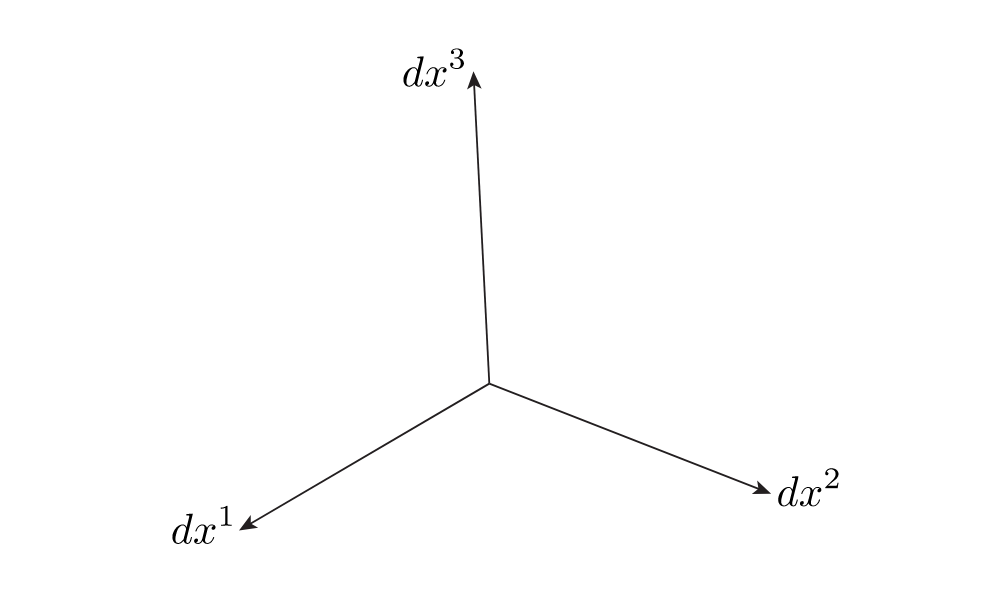
\includegraphics[width=.8\columnwidth]{1forms.png}
%\end{figure}
%\vfill
%\end{frame}
%
%\begin{frame}{2-Forms}
%\begin{figure}[H]
%    \centering
%	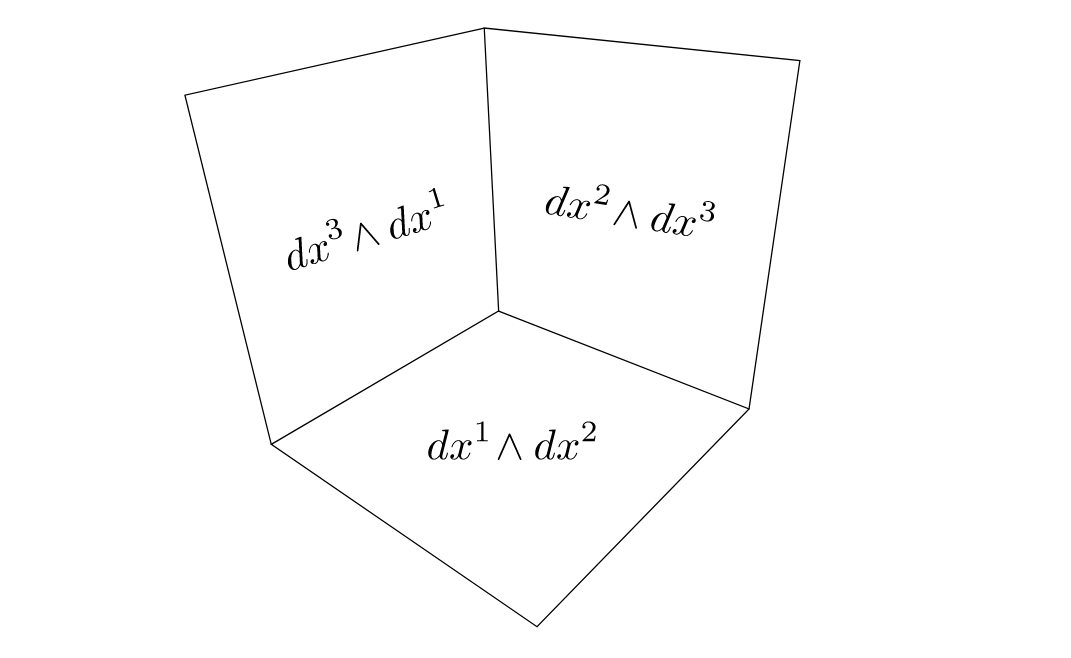
\includegraphics[width=.8\columnwidth]{2forms.png}
%\end{figure}
%\vfill
%\end{frame}
%
%\begin{frame}{3-Forms}
%\vfill
%\begin{figure}[H]
%    \centering
%	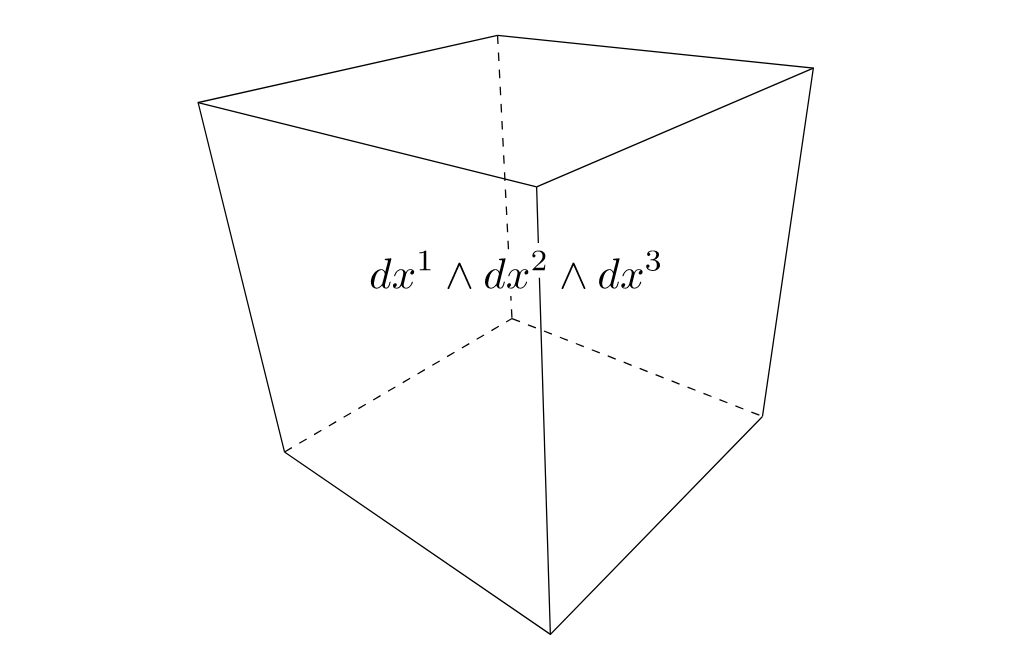
\includegraphics[width=.8\columnwidth]{3forms.png}
%\end{figure}
%\vfill
%\end{frame}
%
%
%
%
%\begin{frame}{Partial Differential Equations}
%    \vfill
%    \pause
%    \begin{itemize}
%    \item \boldgreen{$k$-Form Inner Product}: $\displaystyle{\langle\alpha,\beta\rangle = \int_\Omega \alpha \wedge \star \beta}$.
%    \pause
%
%        \item \boldgreen{Exterior Derivative}: Derivative operator $d$ defined on $k$-forms.
%
%        \pause
%        \item \boldgreen{Codifferential}: Formal adjoint to $d$ written as $\delta$.
%
%        \pause
%        \item \boldgreen{Dirac Operator}: $D=d+\delta$.
%
%        \pause
%        \item \boldgreen{Laplace-Beltrami Operator}: $\Delta = d\delta +\delta d=D^2$ and in coordinates
%        \[
%        \Delta f = \frac{1}{\sqrt{|g|}} \sum_{j=1}^n \sum_{k=1}^n \frac{\partial}{\partial x^i} \sqrt{|g|} g^{ij} \frac{\partial}{\partial x^j} f
%        \]
%    \end{itemize}
%\end{frame}
%
%\subsection{Raphrasing EIT Problem in a Geometrical Language}
%

%
%\subsection{Expected and Current Results}
%
%\begin{frame}{Formal Variable Count}
%    \pause $f \mapsto \Lambda(f)$ approximated by
%    \[
%    \Lambda(f)_j = \sum_{k=1}^m \lambda_{jk} f_k.
%    \]
%
%    \pause In the smooth setting,
%    \[
%    \Lambda(f) = \int_{\partial \Omega} \lambda(x,y) f(y)dS(y).
%    \]
%
%    \pause So, $g$ is a function of $n$ variables that needs to be determined by the kernel $\lambda$ which is $2n-2$ variables.
%\end{frame}
%
%\begin{frame}{Formal Variable Count}
%\vfill
%\begin{itemize}
%    \pause
%    \item $n=1$ gives us an undetermined system.
%
%    \pause
%    \item $n=2$ is well determined.
%
%    \pause
%    \item $n\geq 3$ is overdetermined.
%   \end{itemize}
%\vfill
%\end{frame}
%
%
%
%
%\section{Boundary Control Method in 2 Dimensions}
%
%\begin{frame}{Theorem}
%    \pause
%    \emph{Two $2$-dimensional compact orientable manifolds with single common boundary are conformally equivalent iff their DN-maps coincide.}\\
%
%    \vspace*{1cm}
%    Belishev's \emph{The Calder\'on Problem for Two-Dimensional Manifolds by the BC-Method.}
%\end{frame}
%
%
%\begin{frame}{Key Ideas}
%\vfill
%\pause
%    \begin{itemize}
%        \item Surfaces are two dimensional and can be related to $\C$.
%
%        \pause
%        \item Holomorphic functions have components that are harmonic.
%
%        \pause
%        \item Hilbert transform converts one harmonic function to another by connecting them via a single holomorphic function.
%
%        \pause
%        \item Gelfand transform relates an algebra $\algebra$ to the algebra of continuous functions on the spectrum of that algebra, $C(\spec \algebra)$.
%
%        \pause
%        \item This gives us a way to realize $\Omega$ from functions defined on $\Omega$ that we have access to.
%    \end{itemize}
%\vfill
%\end{frame}
%
%\begin{frame}{Outline of the Proof}
%\vfill
%\pause
%    \begin{itemize}
%        \item From DN map, recover the algebra of holomorphic functions. (Lemma 1)
%
%        \pause
%        \item Show that this algebra is generic. (Lemma 2)
%
%        \pause
%        \item Represent the trace algebra with the DN map. (Lemma 3)
%
%        \pause
%        \item Construct the manifold. (Theorem)
%    \end{itemize}
%\vfill
%\end{frame}
%
%\begin{frame}{Some Notes}
%    \vfill
%    \begin{itemize}
%    \pause
%    \item We have the inclusion of the boundary $\iota \colon \partial \Omega \to \Omega$.
%
%    \pause
%    \item The pullback $\iota^* \colon T^*\Omega \to T^*\partial \Omega$.
%
%    \pause
%    \item Define $\Lambda$ by $\iota^*(\star d u)$ for a harmonic $u$.
%
%    \pause
%    \item $\Lambda$ maps boundary $k$-forms to boundary $n-k-1$ forms.
%    \end{itemize}
%\end{frame}
%
%\begin{frame}{}
%\begin{figure}[H]
%    \centering
%	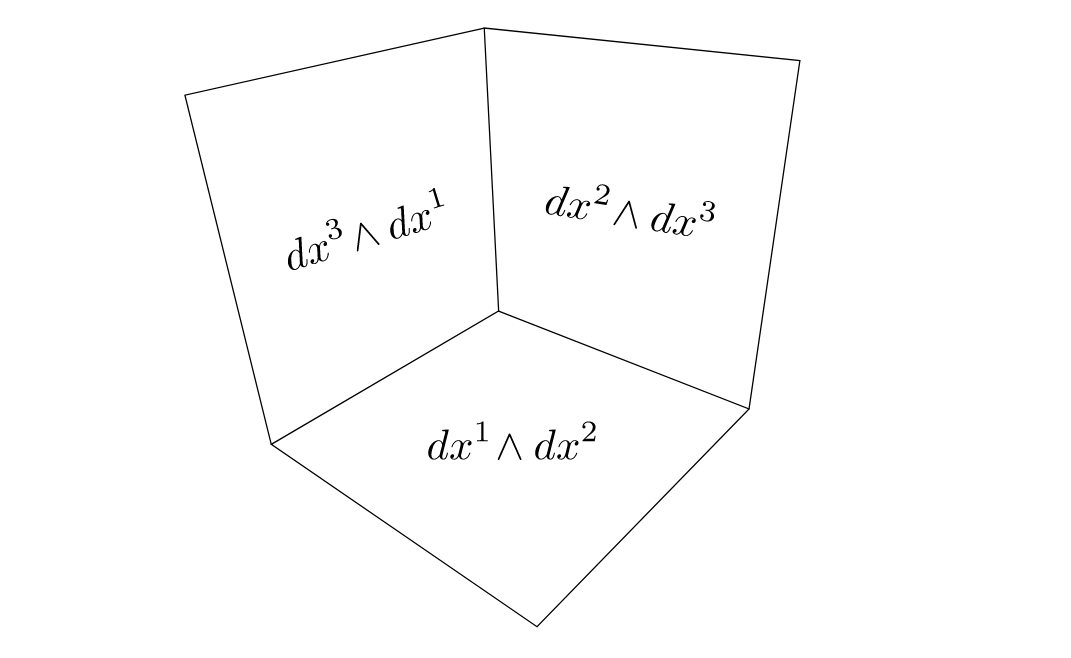
\includegraphics[width=.8\columnwidth]{2forms.png}
%\end{figure}
%\vfill
%\end{frame}
%
%\subsection{Lemma 1}
%
%\begin{frame}{Lemma 1}
%\vfill
%        \begin{itemize}
%            \pause
%            \item A function $u$ satisfying $\Delta u =0$ has a conjugate function $v$ if and only if the trace $\iota^* u$ satisfies
%            \[
%                \left[ \Lambda + d\Lambda^{-1} d\right] \iota^*u = 0.
%            \]
%
%            \pause
%            \item $\dim\textrm{Ran}\left[ \Lambda + d \Lambda^{-1} d \right] = \beta_1(\Omega).$
%        \end{itemize}
%        \vfill
%\end{frame}
%
%\begin{frame}{Corollary}
%\vfill
%    $\Lambda$ completely determines the topology of $\Omega$.
%\vfill
%\end{frame}
%
%\begin{frame}{Proof}
%\vfill
%\pause
%    \begin{itemize}
%        \item Since $\Omega$ is a single connected component, $\beta_0(\Omega)=1$.
%        \item We have $\beta_1(\Omega)$ from before.
%        \item Since $\Omega$ is a surface with boundary, $\beta_2(\Omega)=0$.
%        \item Since $\Omega$ is two dimensional, $\beta_n(\Omega)=0$ for $n\geq 3$.
%    \end{itemize}
%\vfill
%\end{frame}
%
%\begin{frame}{Conjugate Function Intuition}
%\vfill
%\begin{itemize}
%   \pause
%   \item Suppose we have homorphic complex function $w = u + i v$.
%
%   \pause
%   \item Let $u$ be a 0-form and $v$ as a 2-form.
%
%   \pause
%   \item Then $\frac{\partial}{\partial \overline{z}}$ is given by $D=d+\delta$.
%
%   \pause
%   \item $Dw=0$ gives us the Cauchy-Riemann equations
%
%   \item We call $u$ and $v$ conjugate by CREs.
%\end{itemize}
%\vfill
%\end{frame}
%
%\begin{frame}{Hilbert Transform}
%\vfill
%\begin{itemize}
%    \pause
%    \item We can get $v$ from $u$ via the Hilbert transform.
%
%    \pause
%    \item Define $\hilbert = d \Lambda^{-1}$.
%\end{itemize}
%\vfill
%\end{frame}
%
%\begin{frame}{Construct the Algebra $\algebra(\Omega)$}
%\vfill
%\begin{itemize}
%    \pause
%    \item By Lemma 1 we can now create the algebra $\algebra(\Omega)\subset C(\Omega)$ from harmonic functions $u$ with conjugates $v$ by
%    \[
%    \algebra(\Omega) \coloneqq \{ w = u+iv\}.
%    \]
%    Algebra since product of two holomorphic functions is holomorphic.
%
%    \pause
%    \item In isothermal coordinates, each $w\in \algebra(\Omega)$ is holomorphic.
%
%    \pause
%    \item This gives $\Omega$ a complex structure.
%
%    \pause
%    \item This is analogous to having the Hodge star on a surface.
%\end{itemize}
%\vfill
%\end{frame}
%
%\subsection{Lemma 2}
%
%
%\begin{frame}{Gelfand Representation}
%\vfill
%    \begin{itemize}
%    \pause
%            \item Let $\functionals$ be the set of multiplicative linear functionals on a commutative Banach algebra $\algebra$.
%
%        \pause
%        \item The Gelfand transform gives a way of representing an algebra $\algebra$ as a function algebra $\hat{\algebra}$.
%
%        \pause
%        \item The \boldgreen{Gelfand transform} maps $a\in \algebra$ to a function $\hat{a}$ on $\functionals$ by
%        \[
%        \hat{a}(\delta) \coloneqq \delta(a), \quad \delta \in \functionals.
%        \]
%
%        \pause
%        \item The \boldgreen{Gelfand topology} is the weakest topology on $\functionals$ in which all $\hat{a}$ are continuous. This makes $\functionals$ compact.
%
%        \pause
%        \item $\functionals$ with this topology is called the \boldgreen{spectrum} $\spec \algebra$.
%    \end{itemize}
%\vfill
%\end{frame}
%
%\begin{frame}{Generic Algebras}
%\vfill
%    \begin{itemize}
%        \pause
%        \item The Gelfand transform $\hat{\algebra}$ is a subalgebra of $C(\spec \algebra)$ and $a\mapsto \hat{a}$ is an isometric isomorphism.
%
%%        \pause
%%        \item An isomorphism $t\colon A(X) \to B(Y)$ between two function algebras is \boldgreen{spatial} if there exists a bijection $b \colon X \to Y$ such that $tw=w\circ b^{-1}$.
%
%        \pause
%        \item For a function algebra $\algebra \subset C(X)$, take $\epsilon \colon X \to \spec \algebra$ with $\epsilon(x)=\delta_x$.
%
%        \pause
%        \item A function algebra $\algebra \subset C(X)$ is \boldgreen{generic} if $\epsilon$ is a homeomorphism.
%
%        \pause
%        \item A generic algebra is (spatially) isomorphic to its Gelfand transform.
%
%    \end{itemize}
%\vfill
%\end{frame}
%
%\begin{frame}{Lemma 2}
%\vfill
%\pause
%    The algebra of holomorphic functions $\algebra(\Omega)$ is generic.
%\vfill
%\end{frame}
%
%\begin{frame}{Importance}
%\vfill
%    \begin{itemize}
%        \pause
%        \item $\hat{\algebra}(\partial \Omega)$ is (spatially) isomorphic to $\algebra(\Omega)$ by taking the Gelfand transform of the trace.
%
%        \pause
%        \item The lemma shows that $\epsilon \colon \Omega \to \spec \algebra(\Omega)$ is a homeomorphism, so we have determined $\Omega$ up to homeomorphism.
%    \end{itemize}
%\vfill
%\end{frame}
%
%\begin{frame}{What's Left?}
%\vfill
%\pause
%
%    We can only have hope access to the trace algebra $\algebra(\partial \Omega)$. So we need to determine this to reach our goal.
%    \vfill
%\end{frame}

%\begin{frame}{Commutative Banach Algebras (CBA)}
%\vfill
%    \begin{itemize}
%        \pause
%        \item An algebra $\algebra$ is a \boldgreen{commutative Banach Algebra} if
%        \begin{itemize}
%            \item $\algebra$ is a Banach space.
%            \item $a,b \in \algebra$ satisfy $\|ab\|\leq \|a\|\|b\|$.
%        \end{itemize}
%
%        \pause
%        \item $\algebra(\Omega) \subset C(\Omega)$.
%
%        \pause
%        \item $C(\Omega)$ is a CBA and $\algebra(\Omega)$ is a subalgebra.
%
%        \pause
%        \item $C(\Omega)$ is a \boldgreen{uniform} algebra so $\|a^2\|=\|a\|^2$.
%    \end{itemize}
%\vfill
%\end{frame}
%
%\begin{frame}{Ideals and Functionals}
%\vfill
%    \begin{itemize}
%        \pause
%        \item A subspace $I\neq \algebra$ is an \boldgreen{ideal} if $ja \in I$ for $j\in I$ and $a\in \algebra$.
%
%        \pause
%        \item An ideal is \boldgreen{maximal} if $\tilde{I}\subset \algebra$ and $I\subset \tilde{I}$ implies $I=\tilde{I}$.
%
%        \pause
%        \item A functional $\delta \in \algebra'$ is \boldgreen{multiplicative} if $\delta(ab)=\delta(a)\delta(b)$.
%
%        \pause
%        \item Ex: Dirac measure since $\delta_x(ab)=a(x)b(x)$.
%    \end{itemize}
%\vfill
%\end{frame}

%\begin{frame}{Ideals and Functionals}
%\vfill
%    \begin{itemize}
%        \pause
%        \item Let $\ideals$ be the set of maximal ideals of $\algebra$.
%
%        \pause
%        \item Let $\functionals$ be the set of multiplicative functions on $\algebra$.
%
%        \pause
%        \item These sets are in bijection.
%
%        \begin{itemize}
%            \item If $\delta \in \functionals$ then $I_\delta \coloneqq \ker \delta \in \ideals$.
%            \item If $I\in \ideals$ then $\delta_I \colon \algebra \to \algebra / I = \C$ is in $\functionals$.
%        \end{itemize}
%    \end{itemize}
%\vfill
%\end{frame}






%\subsection{Lemma 3}
%
%\begin{frame}{Trace Algebra}
%\vfill
%    \begin{itemize}
%        \pause
%        \item The trace algebra $\algebra (\partial \Omega) \coloneqq \iota^* \algebra(\Omega)$ is isometrically isomorphic to $\algebra(\Omega)$ since
%        \[
%        \|w\|_{\algebra(\Omega)} = \|\iota^* w \|_{\algebra(\partial \Omega)}
%        \]
%        and since a holomorphic function is uniquely determined by its boundary values.
%    \end{itemize}
%\vfill
%\end{frame}
%
%\begin{frame}{Lemma 3}
%\vfill
%    We have the representation
%    \[
%    \algebra(\partial \Omega) = \mathrm{clos}_{C(\partial \Omega)} \{ f +i h\},
%    \]
%    where $h$ is conjugate to $f$ by $\hilbert$.
%\vfill
%\end{frame}
%
%\subsection{Proof of the Main Theorem}
%
%
%\begin{frame}{Construction of the Manifold}
%\vfill
%\pause
%Following these steps yields a manifold $(\Omega, g)$ with the DN map $\Lambda$.
%    \begin{itemize}
%        \pause
%        \item \underline{Step 1:} We know $g|_{\partial \Omega}$ by Lee and Uhlmann, and thus we know $\hilbert$ and $C^\infty(\partial \Omega)$.  This allows us to recover the trace algebra $\algebra(\partial \Omega)$ using the representation in Lemma 3.
%
%        \pause
%        \item \underline{Step 2:} Then find $\spec \algebra(\partial \Omega)=\Omega$ by Lemma 2.
%
%        \pause
%        \item \underline{Step 3:} Next, the Gelfand transform $\hat{\algebra}(\partial \Omega)=\algebra(\Omega)$ by Lemma 2.
%
%        \pause
%        \item \underline{Step 4:} $\algebra(\Omega)$ gives us the complex structure on $\Omega$ by Lemma 1.
%
%        \pause
%        \item \underline{Step 5:} Equip $\Omega$ with a metric $g$ conforming to this complex structure.
%    \end{itemize}
%\vfill
%\end{frame}
%
%
%
%
%\section{Generalizing This Method}
%
%\begin{frame}{First Issue}
%\vfill
%\pause
%    \begin{itemize}
%        \item No complex structure in higher dimensions.
%    \end{itemize}
%    \vfill
%\end{frame}
%
%\begin{frame}{Resolution}
%\vfill
%\pause
%    \begin{itemize}
%        \item Use a Clifford algebra/calculus structure to replace $\C$.
%
%        \pause
%        \item The tools of Clifford analysis allow us to recover a notion of holomorphicity known as \boldgreen{monogenicity}.
%
%        \pause
%        \item We can recover a similar algebra (Hardy space) of monogenic functions.
%    \end{itemize}
%\vfill
%\end{frame}
%
%\begin{frame}{Clifford Structure}
%\vfill
%    A Clifford algebra builds upon the exterior algebra of forms.  Given a quadratic space $(V,Q)$, we have
%    \pause
%    \begin{itemize}
%        \item The quotient of the tensor algebra
%        \[
%        \clifford(V,Q) =\quotient{\bigoplus_{j=0}^\infty V^{\otimes j}}{\langle v \otimes v - Q(v)\rangle}.
%        \]
%
%        \pause
%        \item If $Q=g$ is an inner product, this yields a geometric product on vectors $u,v \in \clifford(V,g)$
%        \[
%        uv = g(u,v) + u\wedge v.
%        \]
%
%        \pause
%        \item Geometric product can be extended to multivectors.
%    \end{itemize}
%\vfill
%\end{frame}
%
%\begin{frame}{Familiar Examples}
%\vfill
%\pause
%We have all seen Clifford algebras before.  Indeed,
%\pause
%\begin{itemize}
%    \item $\C \cong \clifford(\R,-\cdot)$.
%
%    \pause
%    \item $\C$ also lives inside of $\clifford(\R^2,\cdot)$ as the even subalgebra. That is,
%    \[
%    x+iy \iff 1x + e_1 \wedge e_2 y,
%    \]
%    where $e_1\wedge e_2$ is the bivector (and psuedoscalar).
%    \pause
%    \item $\mathbb{H}$ lives inside of $\clifford(\R^3,\cdot)$ as the even subalgebra.
%\end{itemize}
%\vfill
%\end{frame}
%
%\begin{frame}{Clifford Analysis}
%\vfill
%\begin{itemize}
%\pause
%
%    \item We can replace $d+\delta$ with the Dirac operator $D$
%    \[
%    D = \sum_{j=1}^n e_j \frac{\partial}{\partial x^j}.
%    \]
%
%    \pause
%    \item $D^2 = \Delta$.
%
%    \pause
%    \item Elements in the kernel of $D$ are monogenic.
%
%    \pause
%    \item Monogenic objects in even subalgebra have components that are harmonic.
%
%    \pause
%    \item There are Cauchy integral and Hilbert transform type operators for $D$ in arbitrary dimension.
%    \end{itemize}
%    \vfill
%\end{frame}
%
%\begin{frame}{Second Issue}
%    In dimensions greater than 2, even subalgebra is noncommutative.
%    \begin{itemize}
%        \pause
%        \item The spectral theory for Belishev's solution required a commutative Banach algebra.
%
%        \pause
%        \item The spectral theory for noncommutative Banach algebras is not as developed.
%
%        \pause
%        \item There is still work to do here to find some way around this.
%    \end{itemize}
%\end{frame}
%
%\section{Conclusion}
%
%\begin{frame}{Main Story}
%    \begin{itemize}
%        \pause
%        \item Calder\'on proposed a useful and challenging problem for both theorists and practicioners.
%
%        \pause
%        \item Advances have been made in both areas.
%
%        \pause
%        \item Ideal results are still not yet obtained.
%    \end{itemize}
%\end{frame}
%
%\begin{frame}{Novel Approach}
%    \begin{itemize}
%        \pause
%        \item Belishev solved the 2D problem using the boundary control method.
%
%        \pause
%        \item It relies heavily on complex analysis and the spectral theory for commutative Banach algebras.
%
%        \pause
%        \item These issues remain if we try to naively generalize this approach.
%    \end{itemize}
%\end{frame}
%
%\begin{frame}{New Input}
%    \begin{itemize}
%        \pause
%        \item Clifford algebras and analysis replace the complex structure in arbitrary dimension.
%
%        \pause
%        \item We can still construct the same algebra of holomorphic functions.
%
%        \pause
%        \item The relevant algebras are noncommutative for dimensions $\geq$ 3.
%
%        \pause
%        \item There are possibly other tools at our disposal that may be able to replace the loss of commutivity.
%    \end{itemize}
%\end{frame}
%
%\begin{frame}{}
%    \vfill
%    \centering \huge{Thank you!}
%    \vfill
%\end{frame}


%\section*{Bibliography}
%
%\begin{frame}{References}
%    \begin{itemize}
%        \item \url{http://www.numdam.org/article/SLSEDP_2012-2013____A13_0.pdf}
%        \item Dirichlet to Neumann operator on differential forms
%        \item 2d bc method
%        \item The HIlbert Transform on a smooth closed hypersurface
%    \end{itemize}
%\end{frame}
